\input{"preamble.tex"}

\addbibresource{Complex\_Analysis\_Qual\_Notes.bib}

\let\Begin\begin
\let\End\end
\newcommand\wrapenv[1]{#1}

\makeatletter
\def\ScaleWidthIfNeeded{%
 \ifdim\Gin@nat@width>\linewidth
    \linewidth
  \else
    \Gin@nat@width
  \fi
}
\def\ScaleHeightIfNeeded{%
  \ifdim\Gin@nat@height>0.9\textheight
    0.9\textheight
  \else
    \Gin@nat@width
  \fi
}
\makeatother

\setkeys{Gin}{width=\ScaleWidthIfNeeded,height=\ScaleHeightIfNeeded,keepaspectratio}%

\title{
\textbf{
    Complex Analysis Qualifying Exam Review
  }
  }







\begin{document}

\date{}
\author{D. Zack Garza}
\maketitle


\newpage

% Note: addsec only in KomaScript
\addsec{Table of Contents}
\tableofcontents
\newpage

\hypertarget{useful-techniques}{%
\section{Useful Techniques}\label{useful-techniques}}

\hypertarget{notation}{%
\subsection{Notation}\label{notation}}

\begin{longtable}[]{@{}ll@{}}
\toprule
\begin{minipage}[b]{(\columnwidth - 1\tabcolsep) * \real{0.64}}\raggedright
Notation\strut
\end{minipage} &
\begin{minipage}[b]{(\columnwidth - 1\tabcolsep) * \real{0.35}}\raggedright
Definition\strut
\end{minipage}\tabularnewline
\midrule
\endhead
\begin{minipage}[t]{(\columnwidth - 1\tabcolsep) * \real{0.64}}\raggedright
\({\mathbb{D}}\coloneqq\left\{{z {~\mathrel{\Big|}~}{\left\lvert {z} \right\rvert} \leq 1}\right\}\)\strut
\end{minipage} &
\begin{minipage}[t]{(\columnwidth - 1\tabcolsep) * \real{0.35}}\raggedright
The unit disc\strut
\end{minipage}\tabularnewline
\begin{minipage}[t]{(\columnwidth - 1\tabcolsep) * \real{0.64}}\raggedright
\({\mathbb{H}}\coloneqq\left\{{x+iy {~\mathrel{\Big|}~}y > 0}\right\}\)\strut
\end{minipage} &
\begin{minipage}[t]{(\columnwidth - 1\tabcolsep) * \real{0.35}}\raggedright
The upper half-plane\strut
\end{minipage}\tabularnewline
\begin{minipage}[t]{(\columnwidth - 1\tabcolsep) * \real{0.64}}\raggedright
\(X_{1\over 2}\)\strut
\end{minipage} &
\begin{minipage}[t]{(\columnwidth - 1\tabcolsep) * \real{0.35}}\raggedright
A ``half version of \(X\)'', see examples\strut
\end{minipage}\tabularnewline
\begin{minipage}[t]{(\columnwidth - 1\tabcolsep) * \real{0.64}}\raggedright
\({\mathbb{H}}_{1\over 2}\)\strut
\end{minipage} &
\begin{minipage}[t]{(\columnwidth - 1\tabcolsep) * \real{0.35}}\raggedright
The first quadrant\strut
\end{minipage}\tabularnewline
\begin{minipage}[t]{(\columnwidth - 1\tabcolsep) * \real{0.64}}\raggedright
\({\mathbb{D}}_{1\over 2}\)\strut
\end{minipage} &
\begin{minipage}[t]{(\columnwidth - 1\tabcolsep) * \real{0.35}}\raggedright
The portion of the first quadrant inside the unit disc\strut
\end{minipage}\tabularnewline
\begin{minipage}[t]{(\columnwidth - 1\tabcolsep) * \real{0.64}}\raggedright
\(S \coloneqq\left\{{x + iy {~\mathrel{\Big|}~}x\in {\mathbb{R}},\, 0<y<\pi}\right\}\)\strut
\end{minipage} &
\begin{minipage}[t]{(\columnwidth - 1\tabcolsep) * \real{0.35}}\raggedright
The horizonta strip\strut
\end{minipage}\tabularnewline
\bottomrule
\end{longtable}

\begin{remark}[Showing a function is constant]

If you want to show that a function \(f\) is constant, try one of the
following:

\begin{itemize}
\tightlist
\item
  Write \(f = u + iv\) and use Cauchy-Riemann to show \(u_x, u_y = 0\),
  etc.
\item
  Show that \(f\) is entire and bounded.
\end{itemize}

If you additionally want to show \(f\) is zero, try one of these:

\begin{itemize}
\tightlist
\item
  Show \(f\) is entire, bounded, and \(\lim_{z\to\infty} f(z) = 0\).
\end{itemize}

\end{remark}

\hypertarget{greatest-hits}{%
\subsection{Greatest Hits}\label{greatest-hits}}

Things to know well:

\begin{itemize}
\tightlist
\item
  Estimates for derivatives, mean value theorem
\item
  \cref[CauchyTheorem]{Cauchy's Theorem}
\item
  \cref[CauchyIntegral]{Cauchy's Integral Formula}
\item
  \cref[CauchyInequality]{Cauchy's Inequality}
\item
  \cref[Morera]{Morera's Theorem}
\item
  \cref[SchwarzReflection]{The Schwarz Reflection Principle}
\item
  \cref[MaximumModulus]{Maximum Modulus Principle}
\item
  \cref[SchwarzLemma]{The Schwarz Lemma}
\item
  \cref[Liouville]{Liouville's Theorem}
\item
  \cref[Casorati]{Casorati-Weierstrass Theorem}
\item
  \cref[Rouche]{Rouché's Theorem}
\item
  Properties of linear fractional transformations
\item
  Automorphisms of \({\mathbb{D}}, {\mathbb{C}}, {\mathbb{CP}}^1\).
\end{itemize}

\hypertarget{basic-but-useful-facts}{%
\subsection{Basic but Useful Facts}\label{basic-but-useful-facts}}

\begin{fact}[Some useful facts about basic complex algebra]

\envlist

\begin{itemize}
\item
  \(z\mkern 1.5mu\overline{\mkern-1.5muz\mkern-1.5mu}\mkern 1.5mu = {\left\lvert {z} \right\rvert}^2\)
  \begin{align*}
  \Re(z) = { z + \mkern 1.5mu\overline{\mkern-1.5muz\mkern-1.5mu}\mkern 1.5mu \over 2} && && 
  \Im(z) = {z - \mkern 1.5mu\overline{\mkern-1.5muz\mkern-1.5mu}\mkern 1.5mu \over 2i}
  .\end{align*}
\item
  \(\operatorname{Arg}(z/w) = \operatorname{Arg}(z) - \operatorname{Arg}(w)\).
\item
  Exponential forms of cosine and sine:
  \begin{align*}
  \cos(\theta) = \frac 1 2 \qty{e^{i\theta} + e^{-i\theta}} && &&
  \sin(\theta) = \frac{1}{2i}\qty{e^{i\theta} - e^{-i\theta}}
  .\end{align*}
\item
  Various differentials:
  \begin{align*}
  dz &= dx + i~dy \\
  d\mkern 1.5mu\overline{\mkern-1.5muz\mkern-1.5mu}\mkern 1.5mu &= dx - i~dy \\ \\
  f_z &= f_x = f_y / i
  .\end{align*}
\item
  Integral of a complex exponential:
  \begin{align*}
  \int_{0}^{2 \pi} e^{i \ell x} d x
  &=\left\{\begin{array}{ll}
  {2 \pi} & {\ell=0} \\ 
  {0} & \text{else}
  \end{array}\right.
  .\end{align*}
\end{itemize}

\end{fact}

\begin{fact}[Some useful series]

\begin{align*}
\sum_{k=1}^{n} k &=\frac{n(n+1)}{2} \\
\sum_{k=1}^{n} k^{2} &=\frac{n(n+1)(2 n+1)}{6} \\
\sum_{k=1}^{n} k^{3} &=\frac{n^{2}(n+1)^{2}}{4}  \\
\log(z) &= \sum_{n=0}^\infty { (-1)^n \over n} \qty{z-a}^n \\
{\frac{\partial }{\partial z}\,} \sum_{j=0}^\infty a_j z^j &= \sum_{j=0}^\infty a_{j+1}z^j
\end{align*}

\end{fact}

\hypertarget{advice}{%
\subsection{Advice}\label{advice}}

\begin{itemize}
\tightlist
\item
  Consider \(1/f(z)\) and \(f(1/z)\).
\end{itemize}

\hypertarget{definitions}{%
\section{Definitions}\label{definitions}}

\begin{definition}[Analytic]

A function \(f:\Omega \to {\mathbb{C}}\) is \emph{analytic} at
\(z_0\in \Omega\) iff there exists a power series
\(g(z) = \sum a_n (z-z_0)^n\) with radius of convergence \(R>0\) and a
neighborhood \(U\ni z_0\) such that \(f(z) = g(z)\) on \(U\).

\end{definition}

\begin{definition}[Cauchy-Riemann Equations]

\begin{align*}
u_x = v_y \quad\text{and}\quad u_y = -v_x \\
\frac{\partial u}{\partial r}=\frac{1}{r} \frac{\partial v}{\partial \theta} \quad \text { and } \quad \frac{\partial v}{\partial r}=-\frac{1}{r} \frac{\partial u}{\partial \theta} \\
.\end{align*}

\end{definition}

\begin{definition}[Entire]

A function that is holomorphic on \({\mathbb{C}}\) is said to be
\emph{entire}.

\end{definition}

\begin{definition}[Essential Singularity]

A singularity \(z_0\) is \emph{essential} iff it is neither removable
nor a pole.

Equivalently, a Laurent series expansion about \(z_0\) has a principal
part with infinitely many terms.

\end{definition}

\begin{definition}[Holomorphic]

A function \(f:{\mathbb{C}}\to {\mathbb{C}}\) is \emph{holomorphic} at
\(z_0\) if the following limit converges:
\begin{align*}  
\lim_{h\to 0} {1\over h} \qty{f(z_0 + h) - f(z_0)} \coloneqq f'(z_0)
.\end{align*}

\end{definition}

\begin{definition}[Harmonic]

A real function of two variables \(u(x, y)\) is \emph{harmonic} iff its
Laplacian vanishes:
\begin{align*}  
\Delta u \coloneqq\qty{{\frac{\partial ^2}{\partial x^2}\,} + {\frac{\partial ^2}{\partial y^2}\,}}u = 0
.\end{align*}

\end{definition}

\begin{definition}[Meromorphic]

A function \(f:\Omega\to{\mathbb{C}}\) is \emph{meromorphic} iff there
exists a sequence \(\left\{{z_n}\right\}\) such that

\begin{itemize}
\tightlist
\item
  \(\left\{{z_n}\right\}\) has no limit points in \(\Omega\).
\item
  \(f\) is holomorphic in \(\Omega\setminus\left\{{z_n}\right\}\).
\item
  \(f\) has poles at the points \(\left\{{z_n}\right\}\).
\end{itemize}

If \(f\) is either holomorphic or has a pole at \(z=\infty\) is said to
be meromorphic on \({\mathbb{CP}}^1\).

\end{definition}

\begin{definition}[Poles (and associated terminology)]

A \emph{pole} \(z_0\) of a meromorphic function \(f(z)\) is a zero of
\(g(z) \coloneqq{1\over f(z)}\). If there exists an \(n\) such that
\begin{align*}  
\lim_{z\to z_0}\qty{z-z_0}^nf(z)
\end{align*}
is holomorphic and nonzero in a neighborhood of \(z_0\), then the
minimal such \(n\) is the \emph{order} of the pole. A pole of order 1 is
said to be a \emph{simple pole}.

The pole \(z_0\) is \emph{isolated} iff there exists a neighborhood of
\(z_0\) containing no other poles of \(f\).

\end{definition}

\begin{definition}[Principal Part and Residue]

In a Laurent series
\(f(z) \coloneqq\sum_{n\in {\mathbb{Z}}} c_n (z-z_0)^n\), the
\emph{principal part of \(f\) at \(z_0\)} consists of terms with
negative degree:
\begin{align*}  
P_f(z) \coloneqq\sum_{n=1}^\infty c_{-n}(z-z_0)^{-n}
.\end{align*}

The \emph{residue} of \(f\) at \(z_0\) is the coefficient \(c_{-1}\).

\end{definition}

\begin{definition}[Removable Singularities]

If \(z_0\) is a singularity of \(f\) and there exists a \(g\) such that
\(f(z) = g(z)\) for all \(z\) in some deleted neighborhood
\(U\setminus\left\{{z_0}\right\}\), then \(z_0\) is a \emph{removable
singularity} of \(f\).

\end{definition}

\begin{definition}[Linear Fractional Transformation]

A map of the following form is a \emph{linear fractional
transformation}:
\begin{align*}  
T(z) = {az + b \over cz + d}
,\end{align*}
where the denominator is assumed to not be a multiple of the numerator.

These have inverses given by
\begin{align*}  
T^{-1}(w) = {dw-b \over -cw + a}
.\end{align*}

\end{definition}

\begin{definition}[Conformal Map / Biholomorphism]

A bijective holomorphic map is a \textbf{conformal} (or
angle-preserving) map, a.k.a. a \textbf{biholomorphism}.

Note that some authors just require the weaker condition that
\(f'(z) \neq 0\) for any point.

\end{definition}

\hypertarget{theorems}{%
\section{Theorems}\label{theorems}}

\hypertarget{basics}{%
\subsection{Basics}\label{basics}}

\begin{example}[holomorphic vs non-holomorphic]

\envlist

\begin{itemize}
\tightlist
\item
  \(f(z) = {1\over z}\) is holomorphic on
  \({\mathbb{C}}\setminus\left\{{0}\right\}\).
\item
  \(f(z) = \mkern 1.5mu\overline{\mkern-1.5muz\mkern-1.5mu}\mkern 1.5mu\)
  is \emph{not} holomorphic, since
  \(\mkern 1.5mu\overline{\mkern-1.5muh\mkern-1.5mu}\mkern 1.5mu \over h\)
  does not converge (but is real differentiable).
\end{itemize}

\end{example}

\begin{theorem}[Green's Theorem]

If \(\Omega \subseteq {\mathbb{C}}\) is bounded with
\({{\partial}}\Omega\) piecewise smooth and
\(f, g\in C^1(\mkern 1.5mu\overline{\mkern-1.5mu\Omega\mkern-1.5mu}\mkern 1.5mu)\),
then
\begin{align*}\int_{{{\partial}}\Omega} f\, dx + g\, dy = \iint_{\Omega} \qty{ {\frac{\partial g}{\partial x}\,} - {\frac{\partial f}{\partial y}\,} } \, dA.\end{align*}

\end{theorem}

\begin{theorem}[Summation by Parts]

Define the forward difference operator \(\Delta f_k = f_{k+1} - f_k\),
then
\begin{align*}
\sum_{k=m}^n f_k \Delta g_k  + \sum_{k=m}^{n-1} g_{k+1}\Delta f_k = f_n g_{n+1} - f_m g_m
\end{align*}

\begin{quote}
Note: compare to
\(\int_a^b f \, dg + \int_a^b g\, df = f(b) g(b) - f(a) g(a)\).
\end{quote}

\end{theorem}

\hypertarget{holomorphic-and-entire-functions}{%
\subsection{Holomorphic and Entire
Functions}\label{holomorphic-and-entire-functions}}

\hypertarget{key-theorems}{%
\subsubsection{Key Theorems}\label{key-theorems}}

\begin{theorem}[Cauchy's Theorem]\label{CauchyTheorem}

If \(f\) is holomorphic on \(\Omega\), then
\begin{align*}  
\int_{{{\partial}}\Omega} f(z) \, dz = 0
.\end{align*}

\begin{quote}
Slogan: closed path integrals of holomorphic functions vanish.
\end{quote}

\end{theorem}

\begin{theorem}[Morera's Theorem]\label{Morera}

If \(f\) is continuous on a domain \(\Omega\) and \(\int_T f = 0\) for
every triangle \(T\subset \Omega\), then \(f\) is holomorphic.

\begin{quote}
Slogan: if every integral along a triangle vanishes, implies
holomorphic.
\end{quote}

\end{theorem}

\begin{theorem}[Maximum Modulus]\label{MaximumModulus}

If \(f\) is holomorphic and nonconstant on an open connected region
\(\Omega\), then \({\left\lvert {f} \right\rvert}\) can not attain a
maximum on \(\Omega\). If \(\Omega\) is bounded and \(f\) is continuous
on
\(\mkern 1.5mu\overline{\mkern-1.5mu\Omega\mkern-1.5mu}\mkern 1.5mu\),
then
\(\max_{\mkern 1.5mu\overline{\mkern-1.5mu\Omega\mkern-1.5mu}\mkern 1.5mu} {\left\lvert {f} \right\rvert}\)
occurs on \({{\partial}}\Omega\). Conversely, if \(f\) attains a local
supremum at \(z_0 \in \Omega\), then \(f\) is constant on \(\Omega\).

\end{theorem}

\begin{theorem}[Liouville's Theorem]\label{Liouville}

If \(f\) is entire and bounded, \(f\) is constant.

\end{theorem}

\begin{theorem}[Cauchy Integral Formula]\label{CauchyIntegral}

Suppose \(f\) is holomorphic on \(\Omega\), then
\begin{align*}
f(z) = {1 \over 2\pi i} \oint_{{{\partial}}\Omega} {f(\xi) \over \xi-z}\,d\xi
\end{align*}
and
\begin{align*}
{\frac{\partial ^nf }{\partial z^n}\,}(z) = {n! \over 2\pi i} \int_{{{\partial}}\Omega} {f(\xi) \over (\xi - z)^{n+1}} \,d\xi
.\end{align*}

\end{theorem}

\begin{theorem}[Cauchy's Inequality]\label{CauchyInequality}

For \(z_0 \in D_R(z_0) \subset \Omega\), we have
\begin{align*}
{\left\lvert { f^{(n)} (z_0) } \right\rvert} 
\leq \frac{n !}{2 \pi} \int_{0}^{2 \pi} \frac{ {\left\lVert {f} \right\rVert}_{\infty} } {R^{n+1}} R \,d\theta
= \frac{n !{\left\lVert {f} \right\rVert}_{\infty}}{R^n} 
,\end{align*}
where
\({\left\lVert {f} \right\rVert}_{\infty}\coloneqq\sup_{z\in C_R} {\left\lvert {f(z)} \right\rvert}\).

\begin{slogan}

The \(n\)th Taylor coefficient of an analytic function is at most
\(\sup_{{\left\lvert {z} \right\rvert} = R} {\left\lvert {f} \right\rvert}/R^n\).

\end{slogan}

\end{theorem}

\begin{theorem}[Argument Principle]

For \(f\) meromorphic in \(\gamma^\circ\), if \(f\) has no poles and is
nonvanishing on \(\gamma\) then
\begin{align*}  
\Delta_\gamma \arg f(z) = \int_\gamma {f'(z) \over f(z)} \,dz = 2\pi (Z_f - P_f)
,\end{align*}
where \(Z_f\) and \(P_f\) are the number of zeros and poles respectively
enclosed by \(\gamma\), counted with multiplicity.

\end{theorem}

\begin{theorem}[Rouché's Theorem]\label{Rouche}

If \(f, g\) are analytic on a domain \(\Omega\) with finitely many zeros
in \(\Omega\) and \(\gamma \subset \Omega\) is a closed curve
surrounding each point exactly once, where
\({\left\lvert {g} \right\rvert} < {\left\lvert {f} \right\rvert}\) on
\(\gamma\), then \(f\) and \(f+g\) have the same number of zeros.

Alternatively:

Suppose \(f = g + h\) with \(g \neq 0, \infty\) on \(\gamma\) with
\({\left\lvert {g} \right\rvert} > {\left\lvert {h} \right\rvert}\) on
\(\gamma\). Then
\begin{align*}\Delta_\gamma \arg(f) = \Delta_\gamma \arg(h)\quad\text{ and } Z_f - P_f = Z_g - P_g.\end{align*}

\end{theorem}

\begin{theorem}[The Residue Theorem]

If \(f\) is holomorphic on an open set \(\Omega\) containing a curve
\(\gamma\) and its interior \(\gamma^\circ\), except for finitely many
poles \(\left\{{z_k}\right\}_{k=1}^N \subset \gamma^\circ\). Then
\begin{align*}  
\int_\gamma f(z) \,dz = 2\pi i \sum_{k=1}^N \mathop{\mathrm{Res}}_{z_k} f
.\end{align*}

\end{theorem}

\begin{theorem}[Cayley Transform]

The fractional linear transformation given by
\(F(z) = {i - z \over i + z}\) maps \({\mathbb{D}}\to {\mathbb{H}}\)
with inverse \(G(w) = i {1-w \over 1 + w}\).

\end{theorem}

\begin{theorem}[Schwarz Lemma]\label{SchwarzLemma}

If \(f: {\mathbb{D}}\to {\mathbb{D}}\) is holomorphic with \(f(0) = 0\),
then

\begin{enumerate}
\def\labelenumi{\arabic{enumi}.}
\tightlist
\item
  \({\left\lvert {f(z)} \right\rvert} \leq {\left\lvert {z} \right\rvert}\)
  for all \(z\in {\mathbb{D}}\)
\item
  \({\left\lvert {f'(0)} \right\rvert} \leq 1\).
\end{enumerate}

Moreover, if
\({\left\lvert {f(z_0)} \right\rvert} = {\left\lvert {z_0} \right\rvert}\)
for any \(z_0\in {\mathbb{D}}\) or
\({\left\lvert {f'(0)} \right\rvert} = 1\), then \(f\) is a rotation

\end{theorem}

\begin{theorem}[Mean Value Theorem for Holomorphic Functions]

\begin{align*}
f(z_0) = {1\over \pi r^2} \iint_{D_r(z_0)} f(z)\, dA
.\end{align*}

\end{theorem}

\begin{theorem}[Schwarz Reflection ]\label{SchwarzReflection}

If \(f\) is continuous and holomorphic on \({\mathbb{H}}^+\) and
real-valued on \({\mathbb{R}}\), then the extension defined by
\(F(z) = \mkern 1.5mu\overline{\mkern-1.5muf(\mkern 1.5mu\overline{\mkern-1.5muz\mkern-1.5mu}\mkern 1.5mu)\mkern-1.5mu}\mkern 1.5mu\)
for \(z\in {\mathbb{H}}^-\) is a well-defined holomorphic function on
\({\mathbb{C}}\).

\end{theorem}

\begin{theorem}[Classification of Conformal Maps]

There are 8 major types of conformal maps:

\begin{longtable}[]{@{}ll@{}}
\toprule
\begin{minipage}[b]{(\columnwidth - 1\tabcolsep) * \real{0.62}}\raggedright
Type/Domains\strut
\end{minipage} &
\begin{minipage}[b]{(\columnwidth - 1\tabcolsep) * \real{0.37}}\raggedright
Formula\strut
\end{minipage}\tabularnewline
\midrule
\endhead
\begin{minipage}[t]{(\columnwidth - 1\tabcolsep) * \real{0.62}}\raggedright
Translation/Dilation/Rotation\strut
\end{minipage} &
\begin{minipage}[t]{(\columnwidth - 1\tabcolsep) * \real{0.37}}\raggedright
\(z\mapsto e^{i\theta}(cz + h)\)\strut
\end{minipage}\tabularnewline
\begin{minipage}[t]{(\columnwidth - 1\tabcolsep) * \real{0.62}}\raggedright
Sectors to sectors\strut
\end{minipage} &
\begin{minipage}[t]{(\columnwidth - 1\tabcolsep) * \real{0.37}}\raggedright
\(z\mapsto z^n\)\strut
\end{minipage}\tabularnewline
\begin{minipage}[t]{(\columnwidth - 1\tabcolsep) * \real{0.62}}\raggedright
\({\mathbb{D}}_{1\over 2} \to {\mathbb{H}}_{1\over 2}\), the first
quadrant\strut
\end{minipage} &
\begin{minipage}[t]{(\columnwidth - 1\tabcolsep) * \real{0.37}}\raggedright
\(z\mapsto {1+z \over 1-z}\)\strut
\end{minipage}\tabularnewline
\begin{minipage}[t]{(\columnwidth - 1\tabcolsep) * \real{0.62}}\raggedright
\({\mathbb{H}}\to S\)\strut
\end{minipage} &
\begin{minipage}[t]{(\columnwidth - 1\tabcolsep) * \real{0.37}}\raggedright
\(z\mapsto \log(z)\)\strut
\end{minipage}\tabularnewline
\begin{minipage}[t]{(\columnwidth - 1\tabcolsep) * \real{0.62}}\raggedright
\({\mathbb{D}}_{1\over 2} \to S_{1\over 2}\)\strut
\end{minipage} &
\begin{minipage}[t]{(\columnwidth - 1\tabcolsep) * \real{0.37}}\raggedright
\(z\mapsto \log(z)\)\strut
\end{minipage}\tabularnewline
\begin{minipage}[t]{(\columnwidth - 1\tabcolsep) * \real{0.62}}\raggedright
\(S_{1\over 2} \to {\mathbb{D}}_{1\over 2}\)\strut
\end{minipage} &
\begin{minipage}[t]{(\columnwidth - 1\tabcolsep) * \real{0.37}}\raggedright
\(z\mapsto e^{iz}\)\strut
\end{minipage}\tabularnewline
\begin{minipage}[t]{(\columnwidth - 1\tabcolsep) * \real{0.62}}\raggedright
\({\mathbb{D}}_{1\over 2} \to {\mathbb{H}}\)\strut
\end{minipage} &
\begin{minipage}[t]{(\columnwidth - 1\tabcolsep) * \real{0.37}}\raggedright
\(z\mapsto {1\over 2}\qty{z + {1\over z}}\)\strut
\end{minipage}\tabularnewline
\begin{minipage}[t]{(\columnwidth - 1\tabcolsep) * \real{0.62}}\raggedright
\(S_{1\over 2} \to {\mathbb{H}}\)\strut
\end{minipage} &
\begin{minipage}[t]{(\columnwidth - 1\tabcolsep) * \real{0.37}}\raggedright
\(z\mapsto \sin(z)\)\strut
\end{minipage}\tabularnewline
\bottomrule
\end{longtable}

\end{theorem}

\begin{theorem}[Characterization of conformal maps]

Conformal maps \({\mathbb{D}}\to{\mathbb{D}}\) have the form
\begin{align*}
g(z) = \lambda {1-a \over 1 - \mkern 1.5mu\overline{\mkern-1.5mua\mkern-1.5mu}\mkern 1.5mu z}, \quad {\left\lvert {a} \right\rvert} < 1, \quad {\left\lvert {\lambda} \right\rvert} = 1
.\end{align*}

\end{theorem}

\hypertarget{others}{%
\subsubsection{Others}\label{others}}

\begin{theorem}[Riemann Mapping]

If \(\Omega\) is simply connected, nonempty, and not \({\mathbb{C}}\),
then for every \(z_{0}\in \Omega\) there exists a unique conformal map
\(F:\Omega \to {\mathbb{D}}\) such that \(F(z_{0}) = 0\) and
\(F'(z_{0}) > 0\).

Thus any two such sets \(\Omega_{1}, \Omega_{2}\) are conformally
equivalent.

\end{theorem}

\begin{theorem}[Riemann's Removable Singularity Theorem]

If \(f\) is holomorphic on \(\Omega\) except possibly at \(z_0\) and
\(f\) is bounded on \(\Omega\setminus\left\{{z_0}\right\}\), then
\(z_0\) is a removable singularity.

\end{theorem}

\begin{proposition}[Holomorphic functions have harmonic components]

If \(f(z) = u(x, y) + iv(x, y)\) is holomorphic, then \(u, v\) are
harmonic.

\end{proposition}

\begin{proposition}[Holomorphic functions are continuous.]

\(f\) is holomorphic at \(z_0\) iff there exists an
\(a\in {\mathbb{C}}\) such that
\begin{align*}  
f(z_0 + h) - f(z_0) - ah = h \psi(h), \quad \psi(h) \overset{h\to 0}\to 0
.\end{align*}
In this case, \(a = f'(z_0)\).

\end{proposition}

\begin{proposition}[Cauchy-Riemann implies holomorphic]

If \(f = u+iv\) with \(u, v\in C^1({\mathbb{R}})\) satisfying the
Cauchy-Riemann equations on \(\Omega\), then \(f\) is holomorphic on
\(\Omega\) and
\(f'(z) = {\frac{\partial f}{\partial z}\,} = {1 \over 2} \qty{{\frac{\partial }{\partial x}\,} + {1\over i} {\frac{\partial }{\partial y}\,}}f\).

\end{proposition}

\begin{proposition}[Polar Cauchy-Riemann equations]

\begin{align*}  
\frac{\partial u}{\partial r}=\frac{1}{r} \frac{\partial v}{\partial \theta} \quad \text { and } \quad \frac{1}{r} \frac{\partial u}{\partial \theta}=-\frac{\partial v}{\partial r}
.\end{align*}

\end{proposition}

\begin{proof}

\hfill

\begin{concept}

\hfill

\begin{itemize}
\tightlist
\item
  See
  \href{https://users.math.msu.edu/users/shapiro/Teaching/classes/425/crpolar.pdf}{walkthrough
  here}.
\item
  See problem set 1.
\end{itemize}

\end{concept}

\begin{itemize}
\tightlist
\item
  Take derivative along two paths, along a ray with constant angle
  \(\theta_0\) and along a circular arc of constant radius \(r_0\).
\item
  Then equate real and imaginary parts.
\end{itemize}

\end{proof}

\begin{theorem}[Open Mapping]

Any holomorphic non-constant map is an open map.

\end{theorem}

\hypertarget{series-and-analytic-functions}{%
\subsection{Series and Analytic
Functions}\label{series-and-analytic-functions}}

\begin{proposition}[Power Series are Smooth]

Any power series is smooth and its derivatives can be obtained using
term-by-term differentiation.

\end{proposition}

\begin{proposition}[Uniform Convergence of Series]

A series of functions \(\sum_{n=1}^\infty f_n(x)\) converges uniformly
iff
\begin{align*}  
\lim_{n\to \infty} {\left\lVert { \sum_{k\geq n} f_k } \right\rVert}_\infty = 0
.\end{align*}

\end{proposition}

\begin{theorem}[Weierstrass $M\dash$Test]

If \(\left\{{f_n}\right\}\) with \(f_n: \Omega \to {\mathbb{C}}\) and
there exists a sequence \(\left\{{M_n}\right\}\) with
\({\left\lVert {f_n} \right\rVert}_\infty \leq M_n\) and
\(\sum_{n\in {\mathbb{N}}} M_n < \infty\), then
\(f(x) \coloneqq\sum_{n\in {\mathbb{N}}} f_n(x)\) converges absolutely
and uniformly on \(\Omega\).

Moreover, if the \(f_n\) are continuous, by the uniform limit theorem,
\(f\) is again continuous.

\end{theorem}

\begin{proposition}[Exponential is uniformly convergent in discs]

\(f(z) = e^z\) is uniformly convergent in any disc in \({\mathbb{C}}\).

\end{proposition}

\begin{proof}

Apply the estimate
\begin{align*}  
{\left\lvert {e^z} \right\rvert} \leq \sum {{\left\lvert {z} \right\rvert}^n \over n!} = e^{{\left\lvert {z} \right\rvert}}
.\end{align*}
Now by the \(M{\hbox{-}}\)test,
\begin{align*}  
{\left\lvert {z} \right\rvert} \leq R < \infty \implies {\left\lvert {\sum {z^n \over n!}} \right\rvert} \leq e^R < \infty
.\end{align*}

\end{proof}

\begin{proposition}[Checking radius of convergence]

For a power series \(f(z) = \sum a_n z^n\), define \(R\) by
\begin{align*}  
{1\over R}\coloneqq\limsup {\left\lvert {a_n} \right\rvert}^{1\over n}
.\end{align*}

Then \(f\) converges absolutely on
\({\left\lvert {z} \right\rvert} < R\) and diverges on
\({\left\lvert {z} \right\rvert} > R\).

\end{proposition}

\hypertarget{others-1}{%
\subsection{Others}\label{others-1}}

\begin{theorem}[Casorati-Weierstrass]\label{Casorati}

If \(f\) is holomorphic on \(\Omega\setminus\left\{{z_0}\right\}\) where
\(z_0\) is an essential singularity, then for every
\(V\subset \Omega\setminus\left\{{z_0}\right\}\), \(f(V)\) is dense in
\({\mathbb{C}}\).

\begin{quote}
The image of a disc punctured at an essential singularity is dense in
\({\mathbb{C}}\).
\end{quote}

\end{theorem}

\begin{theorem}[Little Picard]

If \(f:{\mathbb{C}}\to {\mathbb{C}}\) is entire and nonconstant, then
\(\operatorname{im}(f)\) is either \({\mathbb{C}}\) or
\({\mathbb{C}}\setminus\left\{{z_0}\right\}\) for some point \(z_0\).

\end{theorem}

\todo{???}

\begin{theorem}[Continuation Principle / Identity Theorem]

If \(f\) is holomorphic on a bounded connected domain \(\Omega\) and
there exists a sequence \(\left\{{z_i}\right\}\) with a limit point in
\(\Omega\) such that \(f(z_i) = 0\), then \(f\equiv 0\) on \(\Omega\).

\begin{quote}
Two functions agreeing on a set with a limit point are equal on a
domain.
\end{quote}

\end{theorem}

\begin{corollary}

The ring of holomorphic functions on a domain in \({\mathbb{C}}\) has no
zero divisors.

\end{corollary}

\begin{proof}

???

\end{proof}

\todo[inline]{Find the proof!}

\begin{proposition}[Injectivity Relates to Derivatives]

If \(z_0\) is a zero of \(f'\) of order \(n\), then \(f\) is
\((n+1)\)-to-one in a neighborhood of \(z_0\).

\end{proposition}

\begin{proof}

?

\end{proof}

\begin{proposition}[Bounded Complex Analytic Functions form a Banach Space]

For \(\Omega\subseteq{\mathbb{C}}\), show that
\(A({\mathbb{C}})\coloneqq\left\{{f: \Omega \to {\mathbb{C}}{~\mathrel{\Big|}~}f\text{ is bounded}}\right\}\)
is a Banach space.

\end{proposition}

\begin{proof}

?

\begin{quote}
Apply Morera's Theorem and Cauchy's Theorem
\end{quote}

\end{proof}

\hypertarget{residues}{%
\section{Residues}\label{residues}}

\begin{remark}

Check: do you need residues? You may be able to just compute an integral

\begin{itemize}
\item
  Directly by parameterization:
  \begin{align*}
  \int_\gamma f = \int_a^b f(z(t))\, z'(t) && \text{for } z(t) \text{ a parameterization of } \gamma
  ,\end{align*}
\item
  Finding a primitive \(F\),
\item
  Writing \(z= z_0 + re^{i \theta }\)
\end{itemize}

\end{remark}

\begin{proof}[of Cauchy's inequality]

\envlist

\begin{itemize}
\tightlist
\item
  Given \(z_0\in \Omega\), pick the largest disc
  \(D_R(z_0) \subset \Omega\) and let \(C_R = {{\partial}}D_R\).
\item
  Then apply the integral formula.
\end{itemize}

\end{proof}

\begin{proposition}[Residues for simple poles (order 1)]

If \(z_0\) is a simple pole of \(f\), then
\begin{align*}  
\mathop{\mathrm{Res}}_{z_0}f = \lim_{z\to z_0} (z-z_0) f(z)
.\end{align*}

\end{proposition}

\begin{example}[Residue of a simple pole (order 1)]

Let \(f(z) = \frac{1}{1+z^2}\), then
\(\mathop{\mathrm{Res}}(i, f) = \frac{1}{2i}\).

\end{example}

\begin{proposition}[For higher order poles]

If \(f\) has a pole \(z_0\) of order \(n\), then
\begin{align*}  
\mathop{\mathrm{Res}}_{z=z_0} f = \lim_{z\to z_0} {1 \over (n-1)!} \qty{{\frac{\partial }{\partial z}\,}}^{n-1} (z-z_0)^n f(z)
.\end{align*}

\end{proposition}

\hypertarget{conformal-maps}{%
\section{Conformal Maps}\label{conformal-maps}}

\begin{fact}

A bijective holomorphic map automatically has a holomorphic inverse.
This can be weakened: an injective holomorphic map satisfies
\(f'(z) \neq 0\) and \(f ^{-1}\) is well-defined on its range and
holomorphic.

\end{fact}

\hypertarget{plane-to-disc}{%
\subsection{Plane to Disc}\label{plane-to-disc}}

\begin{align*}
\phi: {\mathbb{H}}&\to {\mathbb{D}}\\
\phi(z) &= {z - i \over z + i} \qquad f^{-1}(z) = i\qty{1 + w \over 1 - w}
.\end{align*}

\hypertarget{sector-to-disc}{%
\subsection{Sector to Disc}\label{sector-to-disc}}

For
\(S_\alpha \coloneqq\left\{{z\in{\mathbb{C}}{~\mathrel{\Big|}~}0 < \arg(z) < \alpha }\right\}\)
an open sector for \(\alpha\) some angle, first map the sector to the
half-plane:
\begin{align*}
g: S_\alpha &\to {\mathbb{H}}\\
g(z) &= z^{\pi \over \alpha}
.\end{align*}

Then compose with a map \({\mathbb{H}}\to{\mathbb{D}}\):
\begin{align*}
f: S_\alpha &\to {\mathbb{D}}\\
f(z) &= (\phi \circ g)(z) = {z^{\pi\over \alpha} - i \over z^{\pi\over\alpha} + i}
.\end{align*}

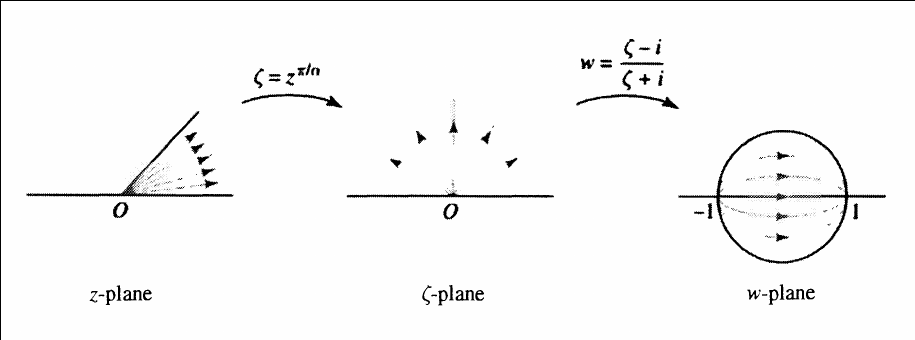
\includegraphics{figures/image_2020-07-22-13-22-46.png}

\hypertarget{strip-to-disc}{%
\subsection{Strip to Disc}\label{strip-to-disc}}

\begin{itemize}
\tightlist
\item
  Map to horizontal strip by rotation \(z\mapsto \lambda z\).
\item
  Map horizontal strip to sector by \(z \mapsto e^z\)
\item
  Map sector to \({\mathbb{H}}\) by \(z\mapsto z^{\pi\over\alpha}\).
\item
  Map \({\mathbb{H}}\to{\mathbb{D}}\).
\end{itemize}

\hypertarget{schwarz-reflection}{%
\section{Schwarz Reflection}\label{schwarz-reflection}}

\begin{remark}

\({\mathbb{H}}^+, {\mathbb{H}}^-\) can be replaced with any region
symmetric about a line segment \(L\subseteq {\mathbb{R}}\).

\end{remark}

\hypertarget{zeros-and-poles}{%
\section{Zeros and Poles}\label{zeros-and-poles}}

\hypertarget{counting-zeros}{%
\subsection{Counting Zeros}\label{counting-zeros}}

\begin{example}

\begin{itemize}
\tightlist
\item
  Take \(P(z) = z^4 + 6z + 3\).
\item
  On \({\left\lvert {z} \right\rvert} < 2\):

  \begin{itemize}
  \tightlist
  \item
    Set \(f(z) = z^4\) and \(g(z) = 6z + 3\), then
    \({\left\lvert {g(z)} \right\rvert} \leq 6{\left\lvert {z} \right\rvert} + 3 = 15 < 16= {\left\lvert {f(z)} \right\rvert}\).
  \item
    So \(P\) has 4 zeros here.
  \end{itemize}
\item
  On \({\left\lvert {z} \right\rvert} < 1\):

  \begin{itemize}
  \tightlist
  \item
    Set \(f(z) = 6z\) and \(g(z) = z^4 + 3\).
  \item
    Check
    \({\left\lvert {g(z)} \right\rvert} \leq {\left\lvert {z} \right\rvert}^4 + 3 = 4 < 6 = {\left\lvert {f(z)} \right\rvert}\).
  \item
    So \(P\) has 1 zero here.
  \end{itemize}
\end{itemize}

\end{example}

\begin{example}

\begin{itemize}
\tightlist
\item
  Claim: the equation \(\alpha z e^z = 1\) where
  \({\left\lvert {\alpha} \right\rvert} > e\) has exactly one solution
  in \({\mathbb{D}}\).
\item
  Set \(f(z) = \alpha z\) and \(g(z) = e^{-z}\).
\item
  Estimate at \({\left\lvert {z} \right\rvert} =1\) we have
  \({\left\lvert {g} \right\rvert} ={\left\lvert {e^{-z}} \right\rvert} = e^{-\Re(z)} \leq e^1 < {\left\lvert {\alpha} \right\rvert} = {\left\lvert {f(z)} \right\rvert}\)
\item
  \(f\) has one zero at \(z_0 = 0\), thus so does \(f+g\).
\end{itemize}

\end{example}

\hypertarget{linear-fractional-transformations}{%
\section{Linear Fractional
Transformations}\label{linear-fractional-transformations}}

\hypertarget{appendix-proofs-of-the-fundamental-theorem-of-algebra}{%
\section{Appendix: Proofs of the Fundamental Theorem of
Algebra}\label{appendix-proofs-of-the-fundamental-theorem-of-algebra}}

\hypertarget{fundamental-theorem-of-algebra-argument-principle}{%
\subsubsection{Fundamental Theorem of Algebra: Argument
Principle}\label{fundamental-theorem-of-algebra-argument-principle}}

\begin{itemize}
\tightlist
\item
  Let \(P(z) = a_nz^n + \cdots + a_0\) and \(g(z) = P'(z)/P(z)\), note
  \(P\) is holomorphic
\item
  Since
  \(\lim_{{\left\lvert {z} \right\rvert} \to \infty} P(z) = \infty\),
  there exist an \(R>0\) such that \(P\) has no roots in
  \(\left\{{{\left\lvert {z} \right\rvert} \geq R}\right\}\).
\item
  Apply the argument principle:
  \begin{align*}     N(0) = {1\over 2\pi i} \oint_{{\left\lvert {\xi} \right\rvert} = R} g(\xi) \,d\xi     .\end{align*}
\item
  Check that
  \(\lim_{{\left\lvert {z\to \infty} \right\rvert}}zg(z) = n\), so \(g\)
  has a simple pole at \(\infty\)
\item
  Then \(g\) has a Laurent series
  \({n\over z} + {c_2 \over z^2} + \cdots\)
\item
  Integrate term-by-term to get \(N(0) = n\).
\end{itemize}

\hypertarget{fundamental-theorem-of-algebra-rouches-theorem}{%
\subsubsection{Fundamental Theorem of Algebra: Rouche's
Theorem}\label{fundamental-theorem-of-algebra-rouches-theorem}}

\begin{itemize}
\tightlist
\item
  Let \(P(z) = a_nz^n + \cdots + a_0\)
\item
  Set \(f(z) = a_n z^n\) and
  \(g(z) = P(z) - f(z) = a_{n-1}z^{n-1} + \cdots + a_0\), so
  \(f+g = P\).
\item
  Choose
  \(R > \max\qty{ { {\left\lvert {a_{n-1}} \right\rvert} + \cdots + {\left\lvert {a_0} \right\rvert} \over {\left\lvert {a_n} \right\rvert} }, 1}\),
  then
\end{itemize}

\begin{align*} |g(z)|  &\coloneqq|a_{n-1}z^{n-1} + \cdots + a_1 z + a_0 | \\ &\leq |a_{n-1}z^{n-1}| + \cdots + |a_1 z| + |a_0 | \quad\text{by the triangle inequality} \\ &= |a_{n-1}|\cdot |z^{n-1}| + \cdots + |a_1|\cdot| z| + |a_0 | \\ &=  |a_{n-1}|\cdot R^{n-1} + \cdots + |a_1| R + |a_0 | \\ &\leq |a_{n-1}|\cdot R^{n-1}+|a_{n-2}|\cdot R^{n-1} + \cdots + |a_1| \cdot R^{n-1} + |a_0 |\cdot R^{n-1} \quad\text{since } R>1 \implies R^{a+b} \geq R^a \\ &= R^{n-1} \left( |a_{n-1}| + |a_{n-2}| + \cdots + |a_1| + |a_0| \right) \\ &\leq R^{n-1} \left( |a_n|\cdot R \right) \quad\text{by choice of } R   \\ &= R^{n} |a_n| \\ &= |a_n z^n| \\ &\coloneqq|f(z)| \end{align*}

\begin{itemize}
\tightlist
\item
  Then \(a_n z^n\) has \(n\) zeros in
  \({\left\lvert {z} \right\rvert} < R\), so \(f+g\) also has \(n\)
  zeros.
\end{itemize}

\hypertarget{fundamental-theorem-of-algebra-liouvilles-theorem}{%
\subsubsection{Fundamental Theorem of Algebra: Liouville's
Theorem}\label{fundamental-theorem-of-algebra-liouvilles-theorem}}

\begin{itemize}
\tightlist
\item
  Suppose \(p\) is nonconstant and has no roots, then \({1\over p}\) is
  entire. We will show it is also bounded and thus constant, a
  contradiction.
\item
  Write
  \(p(z) = z^n \left(a_n + \frac{a_{n-1}}{z}+\dots+\frac{a_{0}}{z^{n}}\right)\)
\item
  Outside a disc:

  \begin{itemize}
  \tightlist
  \item
    Note that \(p(z) \overset{z\to \infty }\to \infty\). so there exists
    an \(R\) large enough such that
    \({\left\lvert {p(z)} \right\rvert} \geq {1\over A}\) for any fixed
    chosen constant \(A\).
  \item
    Then \({\left\lvert { 1/p(z)} \right\rvert} \leq A\) outside of
    \({\left\lvert {z} \right\rvert} >R\), i.e.~\(1/p(z)\) is bounded
    there.
  \end{itemize}
\item
  Inside a disc:

  \begin{itemize}
  \tightlist
  \item
    \(p\) is continuous with no roots and thus must be bounded below on
    \({\left\lvert {z} \right\rvert} < R\).
  \item
    \(p\) is entire and thus continuous, and since
    \(\mkern 1.5mu\overline{\mkern-1.5muD\mkern-1.5mu}\mkern 1.5mu_r(0)\)
    is a compact set, \(p\) achieves a min \(A\) there
  \item
    Set \(C \coloneqq\min(A, B)\), then
    \({\left\lvert {p(z)} \right\rvert} \geq C\) on all of
    \({\mathbb{C}}\) and thus
    \({\left\lvert {1/p(z)} \right\rvert} \leq C\) everywhere.
  \item
    So \(1/p(z)\) is bounded an entire and thus constant by Liouville's
    theorem -- but this forces \(p\) to be constant.
    \({\unicode{x21af}}\)
  \end{itemize}
\end{itemize}

\hypertarget{fundamental-theorem-of-algebra-open-mapping-theorem}{%
\subsubsection{Fundamental Theorem of Algebra: Open Mapping
Theorem}\label{fundamental-theorem-of-algebra-open-mapping-theorem}}

\begin{itemize}
\tightlist
\item
  \(p\) induces a continuous map \({\mathbb{CP}}^1 \to {\mathbb{CP}}^1\)
\item
  The continuous image of compact space is compact;
\item
  Since the codomain is Hausdorff space, the image is closed.
\item
  \(p\) is holomorphic and non-constant, so by the Open Mapping Theorem,
  the image is open.
\item
  Thus the image is clopen in \({\mathbb{CP}}^1\).
\item
  The image is nonempty, since \(p(1) = \sum a_i \in {\mathbb{C}}\)
\item
  \({\mathbb{CP}}^1\) is connected
\item
  But the only nonempty clopen subset of a connected space is the entire
  space.
\item
  So \(p\) is surjective, and \(p^{-1}(0)\) is nonempty.
\item
  So \(p\) has a root.
\end{itemize}

\hypertarget{appendix}{%
\section{Appendix}\label{appendix}}

\hypertarget{misc-basic-algebra}{%
\subsection{Misc Basic Algebra}\label{misc-basic-algebra}}

\begin{fact}[Standard forms of conic sections]

\envlist

\begin{itemize}
\tightlist
\item
  Circle: \(x^2 + y^2 = r^2\)
\item
  Ellipse: \(\qty{\frac x a}^2 + \qty{\frac y b}^2 = 1\)
\item
  Hyperbola: \(\qty{\frac x a}^2 - \qty{\frac y b}^2 = 1\)

  \begin{itemize}
  \tightlist
  \item
    Rectangular Hyperbola: \(xy = \frac{c^2}{2}\).
  \end{itemize}
\item
  Parabola: \(-4ax + y^2 = 0\).
\end{itemize}

Mnemonic: Write \(f(x, y) = Ax^2 + Bxy + Cy^2 + \cdots\), then consider
the discriminant \(\Delta = B^2 - 4AC\):

\begin{itemize}
\tightlist
\item
  \(\Delta < 0 \iff\) ellipse

  \begin{itemize}
  \tightlist
  \item
    \(\Delta < 0\) and \(A=C, B=0 \iff\) circle
  \end{itemize}
\item
  \(\Delta = 0 \iff\) parabola
\item
  \(\Delta > 0 \iff\) hyperbola
\end{itemize}

\end{fact}

\begin{fact}[Completing the square]

\begin{align*}
x^2 - bx = (x - s)^2 - s^2 \quad\text{where} s = \frac{b}{2} \\
x^2 + bx = (x + s)^2 - s^2 \quad\text{where} s = \frac{b}{2}
.\end{align*}

\end{fact}

\begin{fact}

The sum of the interior angles of an \(n{\hbox{-}}\)gon is \((n-2)\pi\),
where each angle is \(\frac{n-2}{n}\pi\).

\end{fact}

Basics

\begin{itemize}
\tightlist
\item
  Show that \({1\over z} \sum_{k=1}^\infty {z^k \over k}\) converges on
  \(S^1 \setminus\left\{{1}\right\}\) using summation by parts.
\item
  Show that any power series is continuous on its domain of convergence.
\item
  Show that a uniform limit of continuous functions is continuous.
\end{itemize}

??

\begin{itemize}
\item
  Show that if \(f\) is holomorphic on \({\mathbb{D}}\) then \(f\) has a
  power series expansion that converges uniformly on every compact
  \(K\subset {\mathbb{D}}\).
\item
  Show that any holomorphic function \(f\) can be uniformly approximated
  by polynomials.
\item
  Show that if \(f\) is holomorphic on a connected region \(\Omega\) and
  \(f'\equiv 0\) on \(\Omega\), then \(f\) is constant on \(\Omega\).
\item
  Show that if \({\left\lvert {f} \right\rvert} = 0\) on
  \({{\partial}}\Omega\) then either \(f\) is constant or \(f\) has a
  zero in \(\Omega\).
\item
  Show that if \(\left\{{f_n}\right\}\) is a sequence of holomorphic
  functions converging uniformly to a function \(f\) on every compact
  subset of \(\Omega\), then \(f\) is holomorphic on \(\Omega\) and
  \(\left\{{f_n'}\right\}\) converges uniformly to \(f'\) on every such
  compact subset.
\item
  Show that if each \(f_n\) is holomorphic on \(\Omega\) and
  \(F \coloneqq\sum f_n\) converges uniformly on every compact subset of
  \(\Omega\), then \(F\) is holomorphic.
\item
  Show that if \(f\) is once complex differentiable at each point of
  \(\Omega\), then \(f\) is holomorphic.
\end{itemize}

\hypertarget{draft-of-problem-book}{%
\section{Draft of Problem Book}\label{draft-of-problem-book}}

\begin{itemize}
\tightlist
\item
  Prove the triangle inequality
\item
  Prove the reverse triangle inequality
\item
  Show that \(\sum z^{k-1}/k\) converges for all \(z\in S^1\) except
  \(z=1\).
\item
  What is an example of a noncontinuous limit of continuous functions?
\item
  Show that the uniform limit of continuous functions is continuous.
\item
  Show that \(f\) is holomorphic if and only if
  \(\mkern 1.5mu\overline{\mkern-1.5mu{\partial}\mkern-1.5mu}\mkern 1.5muf = 0\).
\item
  Show \(n^{1\over n} \overset{n\to \infty } \to 1\).
\item
  Show that if \(f\) is holomorphic with \(f'=0\) on \(\Omega\) then
  \(f\) is constant.
\item
  Show that holomorphic implies analytic.
\item
  Use Cauchy's inequality to prove Liouville's theorem
\end{itemize}

\begin{problem}[?]

What is a pair of conformal equivalences between \({\mathbb{H}}\) and
\({\mathbb{D}}\)?

\begin{solution}

\begin{align*}
F: HH &\to {\mathbb{D}}\\
z & \mapsto {i-z \over i+z}
\\
\\
G: {\mathbb{D}}&\to {\mathbb{H}}\\
w &\mapsto i{1-w \over 1 + w}
.\end{align*}

\begin{quote}
Mnemonic: any point in \({\mathbb{H}}\) is closer to \(i\) than \(-i\),
so \({\left\lvert {F(z)} \right\rvert} < 1\).
\end{quote}

\begin{itemize}
\tightlist
\item
  Maps \({\mathbb{R}}\to S^1\setminus\left\{{-1}\right\}\).
\end{itemize}

\end{solution}

\end{problem}

\begin{problem}[?]

What is conformal equivalence
\({\mathbb{H}}\rightleftharpoons S \coloneqq\left\{{w\in {\mathbb{C}}{~\mathrel{\Big|}~}0 < \arg(w) < \alpha \pi}\right\}\)?

\begin{solution}

\begin{align*}
f(z) = z^ \alpha
.\end{align*}

\end{solution}

\end{problem}


\printbibliography[title=Bibliography]


\end{document}
